\documentclass{article}
\usepackage[pdftex]{graphicx}
\usepackage{pgfplots,wrapfig}
\usepackage{mathtools}
\usepackage{algorithm}
\usepackage[noend]{algpseudocode}
\usepackage{listings}
\usepackage [english]{babel}
\usepackage [autostyle, english = american]{csquotes}
\usepackage{bbold}
\usepackage{braket}
\usepackage{tikz}
\usepackage[margin=1in]{geometry}

\MakeOuterQuote{"}
\newcommand*\Let[2]{\State #1 $\gets$ #2}
\newcommand*\Print[1]{\State \textbf{print} #1}
\newcommand*\Ret{\State \textbf{return}}
\newcommand*\GT[1]{\State \Goto{#1}}
\algnewcommand{\algorithmicgoto}{\textbf{go to}}%
\algnewcommand{\Goto}[1]{\algorithmicgoto~\ref{#1}}%
\newcommand*\rfrac[2]{{}^{#1}\!/_{#2}}
\everymath{\displaystyle}

\usetikzlibrary{trees,calc,arrows.meta,positioning}

\tikzstyle{hollow node}=[circle,draw,inner sep=1.5]
\tikzstyle{solid node}=[circle,draw,inner sep=1.5,fill=black]
\tikzstyle{level 1}=[sibling distance=15mm]
\tikzstyle{level 2}=[sibling distance=25mm]
\tikzstyle{level 3}=[sibling distance=35mm]

\pgfplotsset{compat=1.13}

\definecolor{dkgreen}{rgb}{0,0.6,0}
\definecolor{gray}{rgb}{0.5,0.5,0.5}
\definecolor{mauve}{rgb}{0.58,0,0.82}



\lstset{
	basicstyle=\footnotesize,
	breaklines=true,
	 backgroundcolor=\color{white},   % choose the background color; you must add \usepackage{color} or \usepackage{xcolor}
  basicstyle=\footnotesize,        % the size of the fonts that are used for the code
  breakatwhitespace=false,         % sets if automatic breaks should only happen at whitespace
  breaklines=true,                 % sets automatic line breaking
  captionpos=b,                    % sets the caption-position to bottom
  commentstyle=\color{dkgreen},    % comment style
  deletekeywords={...},            % if you want to delete keywords from the given language
  escapeinside={\%*}{*)},          % if you want to add LaTeX within your code
  extendedchars=true,              % lets you use non-ASCII characters; for 8-bits encodings only, does not work with UTF-8
  frame=single,	                   % adds a frame around the code
  keepspaces=true,                 % keeps spaces in text, useful for keeping indentation of code (possibly needs columns=flexible)
  keywordstyle=\color{blue},       % keyword style
   numbers=left,                    % where to put the line-numbers; possible values are (none, left, right)
  numbersep=5pt,                   % how far the line-numbers are from the code
  numberstyle=\tiny\color{gray}, % the style that is used for the line-numbers
  rulecolor=\color{black},         % if not set, the frame-color may be changed on line-breaks within not-black text (e.g. comments (green here))
  showspaces=false,                % show spaces everywhere adding particular underscores; it overrides 'showstringspaces'
  showstringspaces=false,          % underline spaces within strings only
  showtabs=false,                  % show tabs within strings adding particular underscores
  stepnumber=1,                    % the step between two line-numbers. If it's 1, each line will be numbered
  stringstyle=\color{mauve},     % string literal style
  tabsize=2,	                   % sets default tabsize to 2 spaces
  title=\lstname                   % show the filename of files included with \lstinputlisting; also try caption instead of title
}


\begin{document}

\begin{titlepage}

\begin{center}

\Huge{Homework 1}

\Large{CS 600:  Data Structures and Algorithms }

\Large{Fall 2016}

\Large{John Berlin}



\end{center}

\end{titlepage}
\section*{Question 2}
\begin{lstlisting}[
  mathescape,
  columns=fullflexible,
  basicstyle=\fontfamily{lmvtt}\selectfont,
]
We want to devise a function $NEXTPER(n, \sigma)$ that given an integer
$n$ and a permutation $\sigma$ of $\{1, 2, . . . , n\}$ outputs the ``next permutation''
of $\{1, 2, . . . , n\}$ after $\sigma$ in the lexicographical order. For example, on
an input $(3,\langle1, 3, 2\rangle)$, $NEXTPER$ should output $\langle2, 1, 3\rangle$ and on an
input $(5,\langle2, 3, 5, 4, 1\rangle)$, $NEXTPER$ should output $\langle2, 4, 1, 3, 5\rangle$.
(a) Give pseudocode for the function $NEXTPER$.
(b) Determine the worst case running time of $NEXTPER$.
(c) Implement your pseudocode for $NEXTPER$ using C/C++/Java.
\end{lstlisting}
\subsection*{Answer}
a) 
\textit{Pseudocode} for $NEXTPER(n, \sigma)$

\begin{figure}[h]
\begin{algorithmic}[1]
 \Function{NEXTPER}{$n, \sigma$}
  	\Let{$i,j$}{$n - 1$}
  	\Let{$\sigma'$}{$\sigma$}  
  	\While{$i > 0 \land \sigma'[i-1] \geq \sigma'[i]$}
     	\Let{$i$}{$i - 1$} 
  	\EndWhile
  	\If{$i \leq 0$}
    	\GT{end}
  	\EndIf
 	\While{$\sigma'[j] \leq \sigma'[i-1]$}
      	\Let{$j$}{$j - 1$} 
 	\EndWhile
  	\Let{$\sigma'$}{$swap(\sigma',i-1,j)$}   
 	\Let{$j$}{$n - 1$}
 	\While{$i < j$}
     	\Let{$\sigma'$}{$swap(\sigma',i,j)$}
     	\Let{$i$}{$i + 1$} 
     	\Let{$j$}{$j - 1$} 
  	\EndWhile
  	\Print $\sigma'$ \label{end}
 \EndFunction
\end{algorithmic}

\end{figure}
b) $O(N)$ \newline
To borrow the definition from An introduction to The Design and Analysis of Algorithms edition 2 \cite{Levitin126}
In general, we sean a current permutation from
right to left looking for the first pair of consecutive elements $a_i$ and $a_{i+ 1}$ such that
$a_i < a_{i+1}$ (and, hence, $a_i > \ldots > a_{i+1}$ ). Then we find the smallest element in the
tail that is larger than $a_i$, i.e., $min{a_j | a_j >a_i, j > i}$, and put it in position i; the
positions from $i + 1$ through $n$ are filled with the elements $a_1, a_{1+1},\ldots, a_n$ from
which the element put in the ith position has been eliminated, in increasing order.

But from the code it is clear to see we go through the permutation at most 3 times and from the 
definition we are $O(N)$\newline


\lstinputlisting[language=Java,frame=single,caption={$NEXTPER(n, \sigma)$},label=lst:tw1pr,captionpos=b,numbers=left,showspaces=false,showstringspaces=false,basicstyle=\footnotesize]{src/main/java/jberlin/cs600/odu/edu/Homework1.java} 
\newpage
\section*{Question 3}
\begin{lstlisting}[
  mathescape,
  columns=fullflexible,
  basicstyle=\fontfamily{lmvtt}\selectfont,
]
Give pseudocode for a function $COUNTPERMS(n, \sigma_1 , \sigma_2 )$ that given
an integer n and two permutations $\sigma_1$, $\sigma_2$ of {1, 2, . . . , n} outputs the
number of permutations which come after  $\sigma_1$, but before $\sigma_2$ in the lex-
icographical enumeration. Your function should run in time $O(n^k)$ for
some $k$. Find a function $f(n)$ such that the worst-case running time of
your function $COUNTPERMS(n, \sigma_1 , \sigma_2 )$ is $\Theta(f (n))$.
Hint: Note that we only want to count the number of permutations
between $\sigma_1$ and $\sigma_2$ and not necessarily enumerate them.
\end{lstlisting}
\subsection*{Answer}
\newpage
\section*{Question 4}
\begin{lstlisting}[
  mathescape,
  columns=fullflexible,
  basicstyle=\fontfamily{lmvtt}\selectfont,
]
Prove that for all $k$, $n^k$ is $O(2^n)$
\end{lstlisting}
\subsection*{Answer}
First let me restate the problem, please note I denote ``such that'' as $|$.\newline
Is $f(n)=O(g(n)), \ \forall k$ where $f(n)=n^k ,\ g(n)=2^n$.\newline
To prove this the following properties must hold 
$\{ \exists c  > 0, \ \exists n_0 \ | \ \forall n \geq n_0,  \ 0 \leq f(n) \leq cg(n) \}$.\newline
For this equation $\displaystyle \lim_{n \to \infty}\frac{n^k}{2^n}=0$ thus $0 < \frac{n^k}{2^n} \leq 1$ for some
large $n$.\newline 
Leaving us at $\forall n$ and $n \geq n_0$, $0 < n^k \leq c2^n$ holds and $n^k=O(2^n)$ where $c =1$.\newline
Plugging and chugging  with $n=16,k=2,c=1$ we have $0 \leq 16^2 \leq 1*2^{16} \to 0 \leq 256 \leq 65536$. \newline 
Exactly where we wanted to be, $n^k$ is indeed $O(2^n)$ .

\section*{Question 5}
\begin{lstlisting}[
  mathescape,
  columns=fullflexible,
  basicstyle=\fontfamily{lmvtt}\selectfont,
]
Consider the following idea for sorting a list of size n: Split the list into
$\sqrt{n}$ lists of size $\sqrt{n}$ each, sort each of the smaller list individually and
then merge the sorted lists to get a single sorted list.
(a) Let $T(n)$ denote the worst case running time of an algorithm based
on this idea. Derive a recurrence relation for $T(n)$. Provide a clear
explanation of how you arrived at this recurrence.
(b) Solve the recurrence relation to determine a function $g(n$) such
that $T(n)$ is $\Theta(g(n))$
\end{lstlisting}
\subsection*{Answer}
Part a: \newline
I define the recurrence relation as $ T(n)=\sqrt{n}T(\sqrt{n})+n$.\newline
$n$ or $f(n)$ is the work needed to combined the lists once sorted.\newline
Split the list of size n into $\sqrt{n}$ lists is $T(n)=\sqrt{n}\ldots$\newline
The $\sqrt{n}$ lists get split into $\sqrt{\sqrt{n}}$ sized lists at $T(n)=\sqrt{n}T(\sqrt{n})$ as $T(n)=\sqrt{n}\ldots$ \newline
To better explain consider figure 1 below.
\begin{figure}[h!]
\centering
		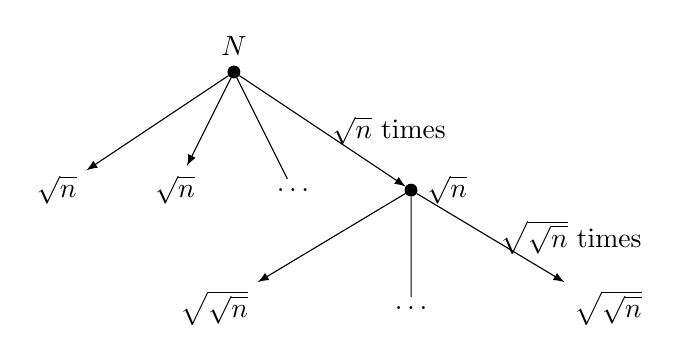
\begin{tikzpicture}
		
		\node(0)[solid node,label=above:{$N$}]{}
		    child { node(1){$\sqrt{n}$} edge from parent[->,>=latex] }
		    child { node(1){$\sqrt{n}$}  edge from parent[->,>=latex]  }
		    child { node(1){$\ldots$}  }
		    child {  
		    	node(1)[solid node,label=right:{$\sqrt{n}$}]{} 
			    child { node(2){$\sqrt{\sqrt{n}}$} edge from parent[->,>=latex]  }
			    child { node(2){{$\ldots$}} }
				child { 
					node(2){$\sqrt{\sqrt{n}}$} edge from parent[->,>=latex] node[right]{$\sqrt{\sqrt{n}}$ times} 
				}
				edge from parent[->,>=latex]  node[right]{$\sqrt{n}$ times}
		    };

		\end{tikzpicture}
		\caption{$T(n)$ expansion}
\end{figure}
\newpage
Part b:\newline
Since this is a variation of merge sort where instead of $\rfrac{1}{2}$ sized lists which is $2T(\rfrac{1}{2})+n$ and is $\Theta(n\log n)$
\newline We are using $ T(n)=\sqrt{n}T(\sqrt{n})+n$ so
\begin{align}
   T(n)&= \begin{aligned}[t]
     \sqrt{n}T(\sqrt{n})+n \\
     \sqrt{n}\left(\sqrt{n}T(\sqrt{\sqrt{n}})+\sqrt{n}\right)+n \\
      \ldots
       \end{aligned}
\end{align}
But ours is similar too merge sort meaning we gotta be somewhere around $\Theta(n\log n)$ so we gotta find our 
$\sqrt{n}T(\sqrt{n})+n \leq cg(n)$. 
Now I will quickly solve (using class notes from merge sort) merge sort so I can use it to solve $ T(n)=\sqrt{n}T(\sqrt{n})+n$.
\begin{align}
   T(n)&= \begin{aligned}[t]
     2T(\frac{n}{2})+n = 2^1T(\frac{n}{2}^{\!1})\\ 
      2^{k-1}T(\frac{n}{2}^{\!k-1})+(k-1)n\\
       2^{k-1} \left( 2T(\frac{n}{2}^{\!k})+\frac{n}{2}^{\!k-1}\right)+(k-1)n \\
       2^kT(\frac{n}{2}^{\!k})+kn \\
       \end{aligned}
\end{align}
Last step $T(n)=nT(1)+n \log n \to n \log n +n$ thus Merge sort is $T(n)=\Theta(n \log n)$. Few...\newline
For  our $ T(n)=\sqrt{n}T(\sqrt{n})+n$ it is clear to see $n \log n$ is way too big for our value of $\Theta$.
Because of the $\sqrt{n}$ step we a definitely somewhere roughly between $n < us < n \log n$ perhaps  $n \log \log n$ or $n \sqrt{\log n}$. I like $n \log \log n$ its a great one plus math.
So by playing algebra king we have:
\begin{align}
   T(n)&=
   \begin{aligned}[t]
   \sqrt{n}T(\sqrt{n})+n \leq \sqrt{n}*c\sqrt{n}\log(\log( \sqrt{n})) + n \\
   \leq c*n\log(\log(n)) - a*n +n \\
   \leq c*n\log(\log(n))
       \end{aligned}
\end{align}
By that $T(n)=\Theta(n\log(\log(n)))$.\newline Revisiting our recursion tree we can see our depth $L$ satisfies $n^{2-L}=2$ \newline ($\sqrt{2}$ does not allow for us to get too 1 thus 2) so by that its clear to see $L=\log(\log( n))$ further solidifying $T(n)=\Theta(n\log(\log(n))$
\begin{figure}[h!]
\centering
		\begin{tikzpicture}
		
		\node(0)[solid node,label=above:{$N$}]{}
		    child { node(1){$\sqrt{n}$} edge from parent[->,>=latex] }
		    child { node(1){$\sqrt{n}$}  edge from parent[->,>=latex]  }
		    child { node(1){$\ldots$}  }
		    child {  
		    	node(1)[solid node,label=right:{$\sqrt{n}$}]{} 
			    child { node(2){$\sqrt{\sqrt{n}}$} edge from parent[->,>=latex]  }
			    child { 
			    	node(2){{$\ldots$}} 
			    	child { node(3){$2$} edge from parent[->,>=latex]  }
			    	child { node(3){$2$} edge from parent[->,>=latex]  }
			    	child { node(3){$2$} edge from parent[->,>=latex]  }
			    	child { node(3){$\ldots$}   }			    	
			    	child { node(3){$2$} edge from parent[->,>=latex]  node[right]{$\ldots$ times} }
			    }
				child { 
					node(2){$\sqrt{\sqrt{n}}$} edge from parent[->,>=latex] node[right]{$\sqrt{\sqrt{n}}$ times} 
				}
				edge from parent[->,>=latex]  node[right]{$\sqrt{n}$ times}
		    };

		\end{tikzpicture}
		\caption{Fuller $T(n)$ expansion}
\end{figure}

\newpage
\clearpage
\begin{thebibliography}{9}

\bibitem{Levitin126}
   Anany V. Levitin,
  Introduction to the Design and Analysis of Algorithms (2nd Edition),
  2006,
  Addison-Wesley,
 Reading, MA

\end{thebibliography} 
\end{document} 